\chapter{CMS实验上的喷注标记技术发展介绍}
\label{chap3}
\fontsize{12bp}{14.4pt}

\section{重建喷注的Anti-$k_T$算法}
Jet 聚类算法是分析强子碰撞数据的主要工具之一。
首先我们有一个待处理列表,里面包含所有待处理的物理对象(包括粒子和已经定义的喷注)。接着对于聚类算法,我们要定义两个物理对象i,j之间的距离\(d_{ij}\),还要额外定义每个物理对象i和入射束流B之间的距离$d_{iB}$。这两类距离的定义如下:
\begin{equation}\label{eq:dij}
    d_{ij}=\min(k_{ti}^{2p},k_{tj}^{2p})\frac{\Delta_{ij}^{2}}{R^{2}}
\end{equation}
\begin{equation}\label{eq:diB}
    d_{iB}=k_{ti}^{2p}
\end{equation}
这里$\displaystyle\Delta_{ij}^{2}=(y_{i}-y_{j})^{2}+(\phi_{i}-\phi_{j})^{2}$,并且$k_{ti}$,$y_i$,$\phi_i$分别是横向动量,快度,方位角。%其中$\displaystyle y =\frac{1}{2}\ln{\frac{E+p_z c}{E-p_z c}}$。

聚类算法是这么执行的:
\begin{enumerate}
    \item 在所有的距离中找到最小的距离,如果:
    \begin{enumerate}[(1)]
        \item 最小距离是来自两个物理对象i,j的距离$d_{ij}$,那我们就把这两个物理对象(i,j)从待处理列表中取出,合并定义为新喷注,再放回待处理列表;
        \item 最小距离是来自物理对象i和入射束流B之间的距离$d_{iB}$,那我们就把物理对象i定义为一个喷注,同时把它从待处理列表中移去(表示已处理完)
    \end{enumerate}
    \item 重新计算待处理列表中的所有距离(包含$d_{ij}$和$d_{iB}$两类)并重复1.步骤,直到待处理列表中没有任何物理对象存在。
\end{enumerate}
通过以上算法,我们就得到了粒子流中的所有喷注。

这里还没有完,对于\eqref{eq:dij}和\eqref{eq:diB}中的幂指数2p,如果我们取p=1,这就是常规的kt算法,并且对于任意p>0的取值都有类似的表现,只有p=0的时候才会变成对应的“Cambridge/Aachen”算法。但是p还有一种取值,就是取p<0,这里对于所有p<0的取值,软辐射的行为都是类似的,我们专门取p=-1,并且称之为anti-$k_t$算法,也叫AK算法。

R通常会取0.4,0.8,1.5三个值,分别对应的算法是AK4,AK8,AK15

anti-$k_t$算法与其他算法重建喷注效果比较如下图所示
\begin{figure}[H]
 \centering
 \caption{用anti-$k_t$算法和$k_t$,Cambridge/Aachen,SISCone算法比较得到的逆反应分布。这是用 Pythia 6.4 模拟的双喷注 事件计算的,其中最硬的两个喷注满足$p_T>$并且都位于$\abs{y}<2$。逆反应
对应于两个最硬喷流中每一个的净横向动量变化,这是由于当高亮度LHC堆积被加入事例时非堆积粒子的重新分配(每束交叉时约有25个pp相互作用)。}
 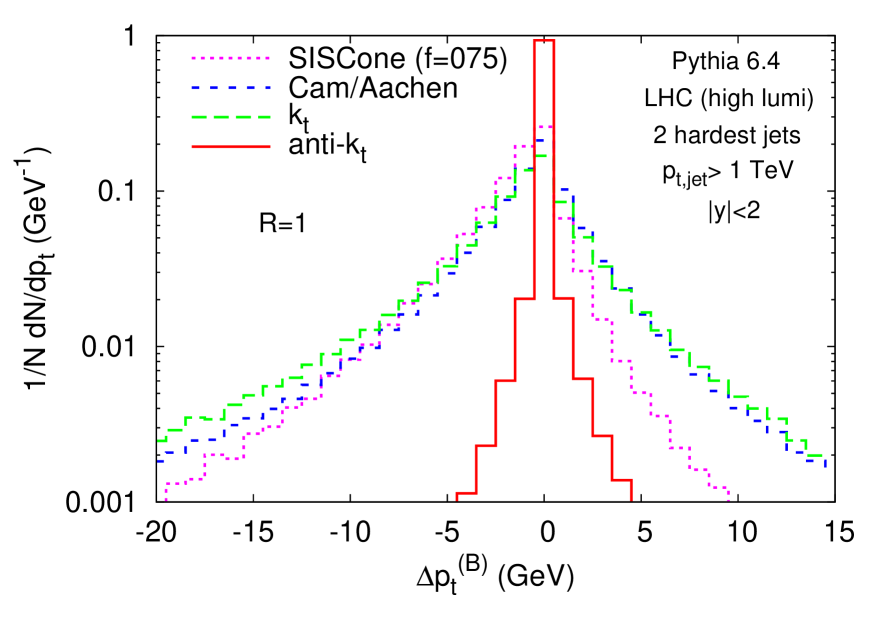
\includegraphics[height=8cm, width=10cm]{pictures/anti-kt.png}
 \label{fig2.1}
\end{figure}


\begin{figure}[H]
 \centering
 \caption{用anti-$k_t$算法和$k_t$,Cambridge/Aachen,SISCone算法比较得到的逆反应分布。这是用 Pythia 6.4 模拟的双喷注 事件计算的,其中最硬的两个喷注满足$p_T>$并且都位于$\abs{y}<2$。逆反应
对应于两个最硬喷流中每一个的净横向动量变化,这是由于当高亮度LHC堆积被加入事例时非堆积粒子的重新分配(每束交叉时约有25个pp相互作用)。}
 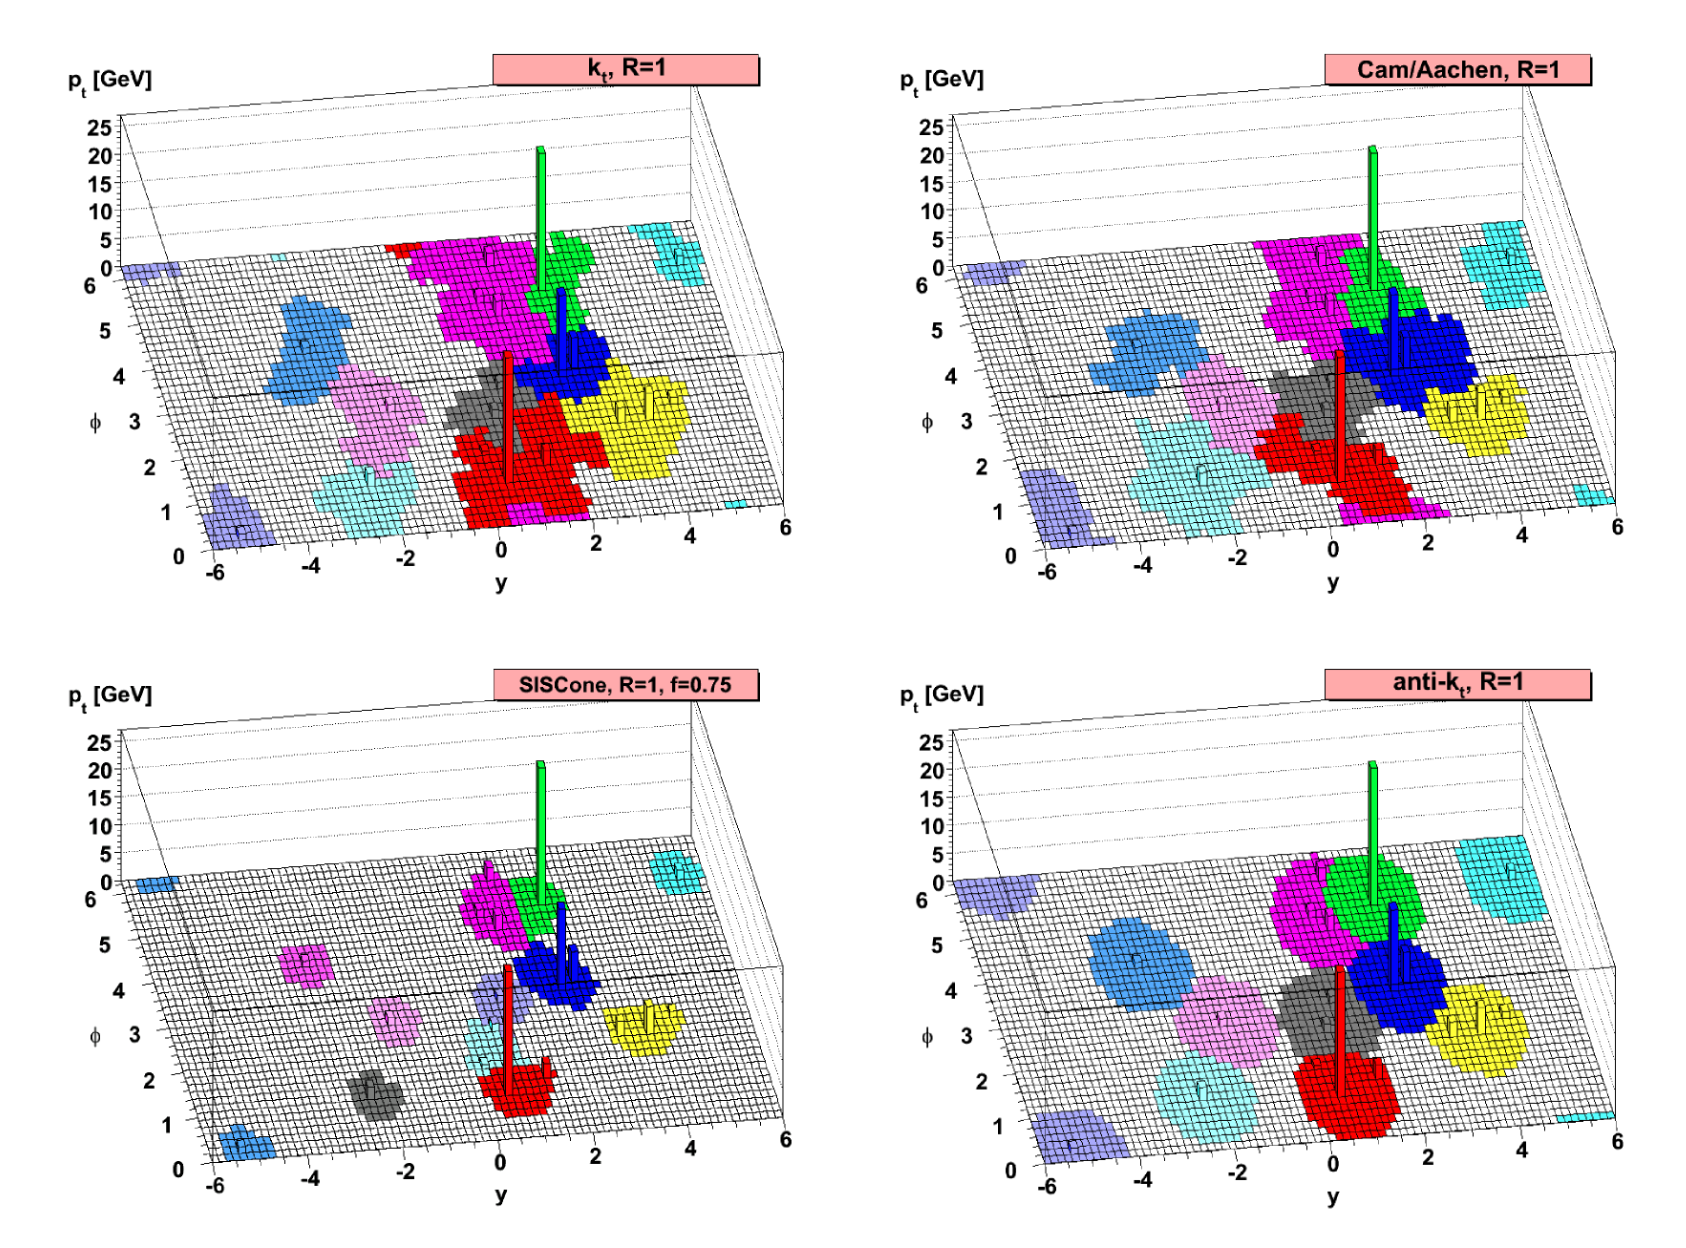
\includegraphics[height=10cm, width=13cm]{pictures/anti-kt-3D.png}
 \label{fig2.2}
\end{figure}

\section{基于理论的高级变量的筛选条件算法}
基于筛选条件的标记算法从理论灵感提供的变量出发,在实验和理论两方面都经受了广泛的研究,具有鲁棒性和易于理解和实现的特点,同时也是与新算法比较的基准线
\subsection{soft-drop mass算法}
我们知道一个喷注由许多的子喷注构成,怎么取舍目标喷注中的子喷注便成了算法的核心问题。

soft-drop算法,就是丢弃掉喷注当中较软且偏离喷注中心较远的子喷注,然后计算剩余较硬且集中在喷注内部的部分的不变质量,其中,剩余的部分子喷注要满足如下的软滴条件:
\begin{itemize}
    \item soft-drop条件:
    \begin{equation}\label{eq:3.1}
        \frac{min(p_{T1}, p_{T2})}{p_{T1}+p_{T2}}>z_{cut} \left(\frac{\Delta R_{12}}{R_0}\right)^\beta
    \end{equation}
\end{itemize}
这里
\begin{equation}\label{eq:3.2}
    R_{12}=\sqrt{(\eta_1-\eta_2)^2+(\phi_1-\phi_2)^2}
\end{equation}
是子喷注1和子喷注2之间的角距离,$R_0$是要求的某个阈值。对于CMS实验,通常我们取$\beta=0$,$z_{cut}=0.1$,soft-drop条件\eqref{eq:3.1}简化为
\begin{equation}
    \frac{min(p_{T1}, p_{T2})}{p_{T1}+p_{T2}}>0.01
\end{equation}
通过soft-drop mass算法,我们可以得到我们想要的子喷注构成的喷注,从而计算出喷注对应的软滴质量(soft drop mass),软滴算法可以大大减少喷注质量分布中的“Sudakov”峰结构,使信号分辨率更明显。
\subsection{N-subjettiness算法}
高级变量N-subjettiness定义为
\begin{equation}
    \tau_N=\frac{1}{d_0}\sum_i p_{T,i}min\left[\Delta R_{1,i},\Delta R_{2,i},\cdots,\Delta R_{N,i}\right]
\end{equation}
这里$\Delta R_{j,i}$是指第j的子喷注到第i个子喷注的角距离。通过$\tau_N$这个变量,我们可以量化一个喷注拥有N个子喷注的兼容性。

进一步地,我们可以通过不同$\tau_N$之间的比值获得更有鉴别效果的变量,例如
\begin{enumerate}[(1)]
    \item 定义
    \begin{equation}
        \tau_{21}=\frac{\tau_2}{\tau_1}
    \end{equation}
    可以针对鉴别二分叉喷注(如W,Z,H)。
    \item 定义
    \begin{equation}
        \tau_{32}=\frac{\tau_3}{\tau_2}
    \end{equation}
    可以针对鉴别三分叉喷注(如top),同时对top喷注的b夸克子喷注还可以运用$\tau_{21}$来进一步改善效果。
\end{enumerate}
在重建中,我们一般在应用soft-drop mass算法后计算喷注的ECF比率,这提高了 ECF 作为喷注质量和$p_T$函数的稳定性。

\subsection{ECF:$N_2$算法}
这里我们要用到泛化能量关联函数(ECF),对于一个包含$N_c$个子喷注的喷注,它的ECF如下定义
\begin{equation}
    {}_{q}e_{N}^{\beta}=\sum_{1\leq i_{1}<i_{2}<\cdots<i_{N}\leq N_{\text{C}}}%
\left[\prod_{1\leq k\leq N}\frac{\pt^{i_{k}}}{\pt^{J}}\right]\prod_{m=1}^{q}%
\min_{i_{j}<i_{k}\in\{i_{1},i_{2},\cdots,i_{N}\}}^{(m)}\left\{\Delta R_{i_{j},%
i_{k}}^{\beta}\right\}
\end{equation}
这个变量可以用来测试喷注有N个辐射中心的兼容性,与N-subjettiness变量有点相似,但是ECF是无轴方法,并且对于N分叉喷注,如果$N>M$,我们会有$e_N\gg e_M$。

对于二分叉标记喷注(W/Z/H),可以定义ECF比值为
\begin{equation}
    N_{2}^{1}=\frac{{}_{2}e_{3}^{1}}{(_{1}e_{2}^{1})^{2}}
\end{equation}
与N-subjettiness比值$\tau_{21}$相比, 其优点是它作为喷注质量和$p_T$的函数更稳定,这种方法也被称为“$m_{SD}+N_2$”算法。

本算法还有质量去相关的版本,便于压低峰状本底,具体做法如下,定义“设计去相关标记器”变量为
\begin{equation}
    N_2^{DDT}(\rho,p_T)=N_2(\rho, p_T)-N_2^{(X\%)}(\rho,p_T)
\end{equation}
此处$\rho=\ln{(m_{SD}^2/p_T^2)}$是一个无量纲变量,$N_2^{(X\%)}$是
模拟QCD样本中$N_2$分布的X百分位的取值。这确保了筛选条件$N^{DDT}_2<0$会导致在考虑的质量与横向动量范围内QCD的标记效率为恒定X\%,并且没有标记性能上的损失。

\section{基于机器学习的高级变量算法}
\subsection{$N_3$-BDT算法}
我们想考虑具有尺度不变性的ECF比率,可以通过以下式子定义的变量来构造:
\begin{equation}
    \frac{{}_{a}e_{N}^{\alpha}}{(_{b}e_{M}^{\beta})^{x}}\text{, where }M\leq N%
\text{ and }x=\frac{a\alpha}{b\beta}.
\end{equation}
对于top夸克喷注标记算法,仅考虑彼此不高度相关的那些变量,并且丢弃无法很好被模拟定义的比值变量,这样我们得到如下11个比值变量
\begin{equation}
\begin{split}
\displaystyle\frac{{}_{1}e_{2}^{(2)}}{\Bigl{(}{}_{1}e_{2}^{(1)}\Bigr{)}^{2}},%
\frac{{}_{1}e_{3}^{(4)}}{{}_{2}e_{3}^{(2)}},\frac{{}_{3}e_{3}^{(1)}}{\Bigl{(}{%
}_{1}e_{3}^{(4)}\Bigr{)}^{3/4}},\displaystyle\frac{{}_{3}e_{3}^{(1)}}{\Bigl{(}{}_{2}e_{3}^{(2)}\Bigr{)}^{3/4}}%
,\frac{{}_{3}e_{3}^{(2)}}{\Bigl{(}{}_{3}e_{3}^{(4)}\Bigr{)}^{1/2}},
\displaystyle\frac{{}_{1}e_{4}^{(4)}}{\Bigl{(}{}_{1}e_{3}^{(2)}\Bigr{)}^{2}},\\
\frac{{}_{1}e_{4}^{(2)}}{\Bigl{(}{}_{1}e_{3}^{(1)}\Bigr{)}^{2}},\frac{{}_{2}e_%
{4}^{(1/2)}}{\Bigl{(}{}_{1}e_{3}^{(1/2)}\Bigr{)}^{2}},\displaystyle\frac{{}_{2}e_{4}^{(1)}}{\Bigl{(}{}_{1}e_{3}^{(1)}\Bigr{)}^{2}},%
\frac{{}_{2}e_{4}^{(1)}}{\Bigl{(}{}_{2}e_{3}^{(1/2)}\Bigr{)}^{2}},\frac{{}_{2}%
e_{4}^{(2)}}{\Bigl{(}{}_{1}e_{3}^{(2)}\Bigr{)}^{2}}.
\end{split}
\end{equation}
基于ECF的top夸克标记器,称为“$N_{3}\text{-}\mathrm{BDT}\,(\mathrm{CA}15)$”,使用扩展决策树模型,以这11个ECF比值变量加上,$\tau^{SD}_{32}\text{和}f_{rec}$作为输入。
\subsection{HOTVR算法}
全称为“带R变量的重对象标记器”(Heavy Object Tagger with Variable R),带$p_T$无关的变量距离参数$R$的喷注簇射和经过Puppi算法修正Pile-up的ParticleFlow候选者,在这个过程中,软簇射会被丢弃掉,从而得到稳定的喷注质量分布,同时阻止额外的辐射进入喷注。

可以被用于标记不同的重共振态(t/W/Z/H)。
\subsection{BEST算法}
全称是“扩展事例形状标记器”(Boosted Event Shape Tagger),是针对top/W/Z/Higgs的多分类标记器,在参考坐标系中计算喷注运动学/形状的变量,,并且把参考坐标系分别按top/W/Z/Higgs喷注假设变换成四个静止坐标系,如果被变换到了正确的静止坐标系,那么喷注的子组分就应该是各向同性并且会展示出预期的N分叉结构。

我们使用神经网络训练这些运动学变量和子喷注的b标记判别式,这个神经网络由三个全连接层构成,每层带有40个节点。
\section{基于深度学习的初级变量算法}
这里实际上已经开始进入深度学习时代,基于深度学习的新标记算法在最近几年已经被提上预案并且受到了大量关注,基本思想就是使用初级变量加上深度神经网络,对于喷注标记,有两种深度神经网络的路径:
\begin{enumerate}[1.]
    \item \textbf{基于图像}:\label{dl:image}\\
    把喷注转化为使用量能器能量沉积得到的图像,利用计算机视觉技术——通常是二维卷积神经网络。但是由于图像的稀疏性和异构探测器,仍然挑战和困难重重。
    \item \textbf{基于粒子}:\label{dl:particle}\\
    把喷注当成它自己组分粒子的集合,这样可以利用循环神经网络,一维卷积神经网络和图神经网络等等技术。同时还可以通过CMS的Particle-Flow重建流程产生诱导出更多自然的想法,合并所有子探测器的信息并且充分利用粒度。
\end{enumerate}

现在这两条算法路径在CMS实验中都在开发,以下将通过两个例子分别介绍这两条路径的情况。
\subsection{IamgeTop算法}
这是基于喷注图像的top夸克标记算法,喷注图像基于喷注横向动量自适应缩放以
增加高$p_T$区域的准直。喷注图像有四个“颜色”通道:(1)中性$p_T$;(2)径迹$p_T$;(3)$\mu$子个数;(4)径迹条数。还运用了深度喷注b夸克标记的判别式。

\textbf{质量去相关的ImageTop算法}:
训练时重新加权QCD样本使得本底的质量分布与top夸克的质量分布相匹配,从而获得ImageTop-MD标记器。
\subsection{DeepAK8算法}
DeepAK8是针对top/W/Z/Higgs标记任务的多分类标记器,其中还会按照衰变道进行进一步的子分类(例如,$Z\to bb$,$Z\to cc$,$Z\to qq$等)。
此算法直接用喷注组分(如ParticleFlow候选者,二级顶点等)作为输入,采用一维卷积神经网络作为架构

\textbf{质量去相关的DeepAK8算法}:
使用对抗训练技术,训练时重新加权本底样本和信号样本获得$m_{SD}$和$p_T$的二维平分布以辅助训练。